\chapter[Occurrence Data]{Occurrence Data, Spatial Cleaning, and Record Preparation}

\begin{objetivos}
By the end of this chapter, readers should be able to identify the main sources
of occurrence data used in species distribution modeling; recognize limitations
of herbarium, inventory, and global-repository data; standardize taxonomic and
geographic records; filter occurrences using the Amazon biome boundary; remove
problematic coordinates, duplicates, and spatially redundant records; apply
spatial thinning; extract environmental values at occurrence locations; and
prepare a final occurrence dataset for subsequent modeling chapters.
\end{objetivos}

\section{Introduction}

Occurrence data provide the empirical foundation of species distribution
modeling. In correlative models, geographic records are associated with the
environmental conditions at locations where a species was observed, making it
possible to estimate occurrence--environment relationships. Model quality,
however, depends directly on the quality of these records.

In real applications, occurrence data may originate from forest inventories,
herbaria, biological collections, digital platforms, scientific literature,
and global repositories such as GBIF. These sources frequently combine
different levels of taxonomic, geographic, and temporal precision. Careful
standardization, cleaning, and spatial filtering are therefore required before
model fitting \parencite{guisan2017habitat,hijmans2021species,zizka2019coordinatecleaner}.

\begin{conceito}[title={\faBook\quad Occurrence record}]
An occurrence record is spatial evidence that a species was present at a given
location. In SDM, it is usually represented by geographic coordinates linked to
the species name, data source, and, when available, date, institution,
collector, and spatial uncertainty.
\end{conceito}

\section{Sources of Occurrence Data}

SDM data can come from several sources. Forest inventories generally provide
stronger taxonomic and spatial control but tend to cover limited areas.
Herbaria and biological collections contain valuable historical records,
although coordinates may be missing or imprecise. Global platforms such as
GBIF increase spatial coverage but require stringent quality filters.

In the reference study used throughout this textbook, records of
\textit{Dinizia excelsa} from inventories and GBIF were integrated and then
subjected to spatial filters, thinning, and extraction of bioclimatic variables
for climatic-niche analysis across Amazonia \parencite{delima2026warmer}. This
chapter implements a comparable workflow.

\begin{dica}[title={\faLightbulb\quad Integrating sources}]
A robust occurrence dataset may combine inventories, herbaria, and GBIF,
provided that every record undergoes standardization, cleaning, and duplicate
control.
\end{dica}

\section{Common Problems in Occurrence Data}

Frequent problems include inconsistent scientific names, invalid coordinates,
marine records for terrestrial species, points located at national or regional
capitals, institutional coordinates, duplicates, reversed latitude and
longitude, georeferencing errors, and strong spatial sampling bias.

For Amazonian species, records are often concentrated near rivers, roads,
cities, herbaria, forest-inventory sites, and logistically accessible regions.
Such patterns do not necessarily indicate greater environmental suitability;
they may instead reflect greater collection effort.

\begin{atencao}[title={\faExclamationTriangle\quad Lack of occurrence is not absence}]
Presence records indicate where a species was observed. A region without
records does not necessarily lack the species; it may simply have received
little or no sampling effort.
\end{atencao}

\section{Data-Preparation Workflow}

The workflow follows the general structure of Amazon-scale SDM studies:
compile records, standardize columns, retain valid coordinates, apply geographic
quality control, crop to the biome, remove duplicates, perform spatial thinning,
extract environmental data, and export the final dataset.

\rscriptfile{scripts/unidade02/01_compilar_ocorrencias_dinizia.R}

\section{Geographic Cleaning and Cropping to the Amazon Biome}

After compilation, records are converted to spatial objects, checked for
coordinate validity, and filtered using the Amazon biome boundary. This step
ensures that the working dataset represents the geographic extent defined for
the study.

\rscriptfile{scripts/unidade02/02_limpeza_espacial_dinizia.R}

\begin{figure}[H]
  \centering
  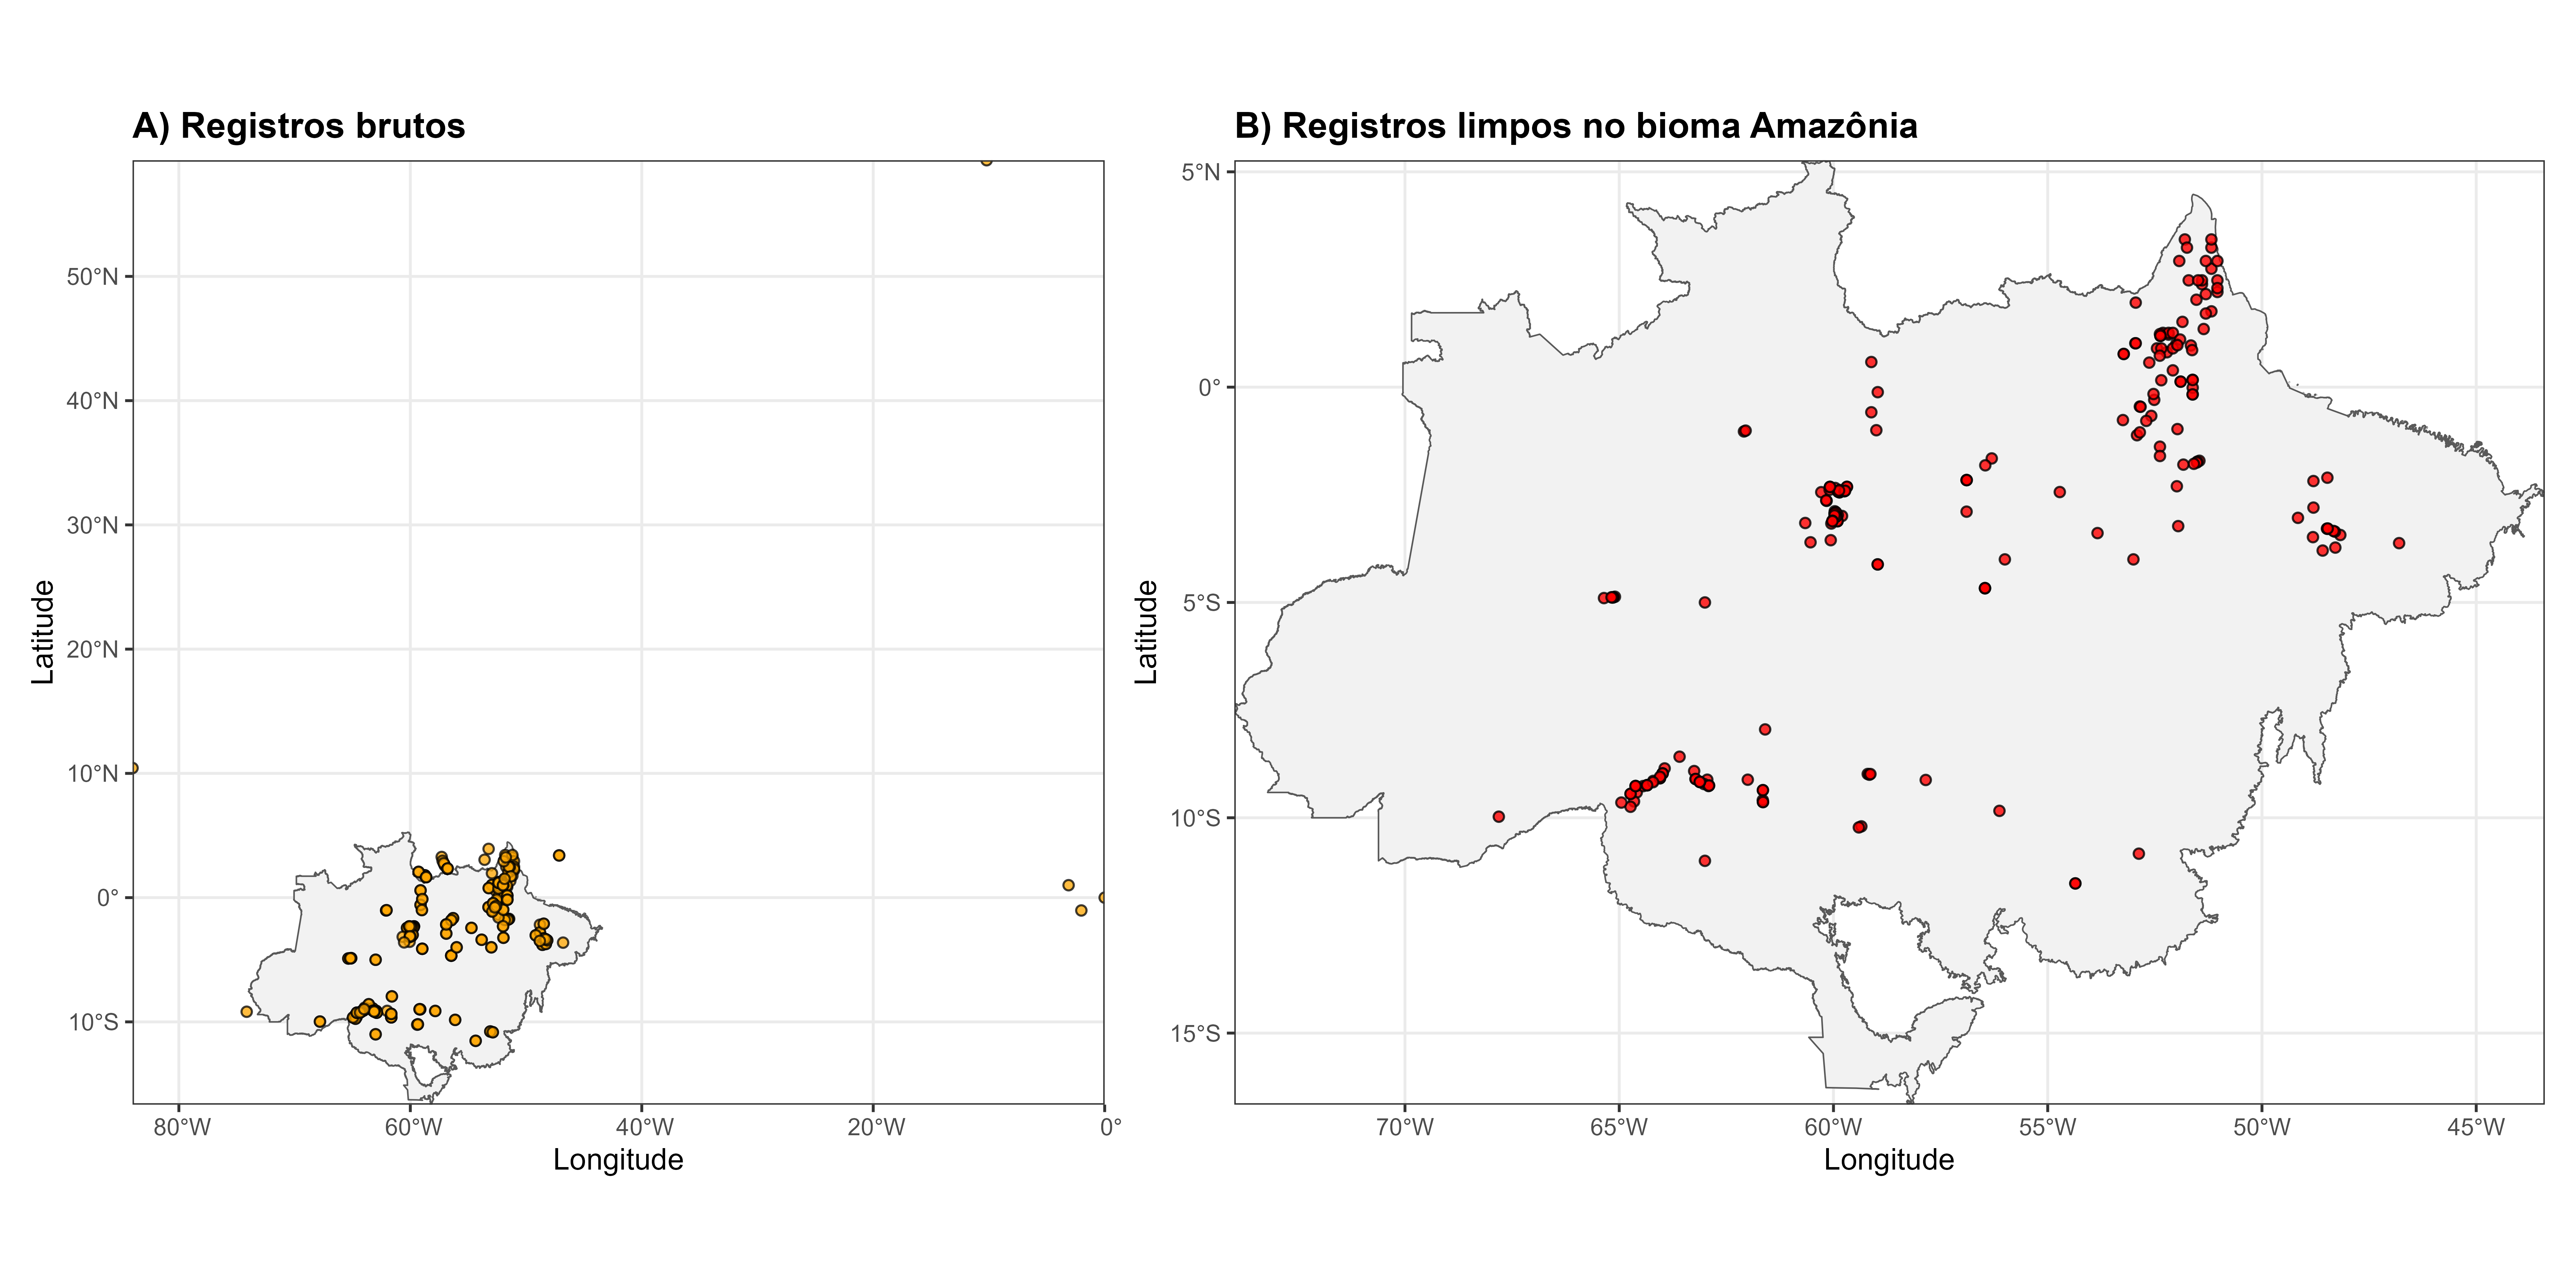
\includegraphics[width=0.92\textwidth]{figuras/unidade02/unidade02_mapa_bruto_limpo_dinizia.png}
  \caption{Comparison of raw and filtered records of \textit{Dinizia excelsa} within the Amazon biome.}
  \label{fig:unidade02_bruto_limpo_dinizia}
\end{figure}

\section{Environmental Extraction and Raster-Cell Duplicates}

Even after identical coordinates have been removed, different records may fall
within the same climatic raster cell. Because models use environmental values
extracted from rasters, multiple points in one cell may constitute environmental
pseudoreplication. It is therefore advisable to retain only one occurrence per
environmental raster cell.

\rscriptfile{scripts/unidade02/03_extrair_ambiente_dinizia.R}

\section{Spatial Thinning}

Spatial thinning reduces excessive concentrations of records in intensively
sampled areas. Here, a minimum distance is imposed between retained
occurrences, helping to reduce spatial autocorrelation and sampling bias. This
procedure is widely used in ecological-niche studies and can be implemented
with the \texttt{spThin} package \parencite{aiellolammens2015spthin}.

\rscriptfile{scripts/unidade02/04_rarefacao_espacial_dinizia.R}

\begin{figure}[H]
  \centering
  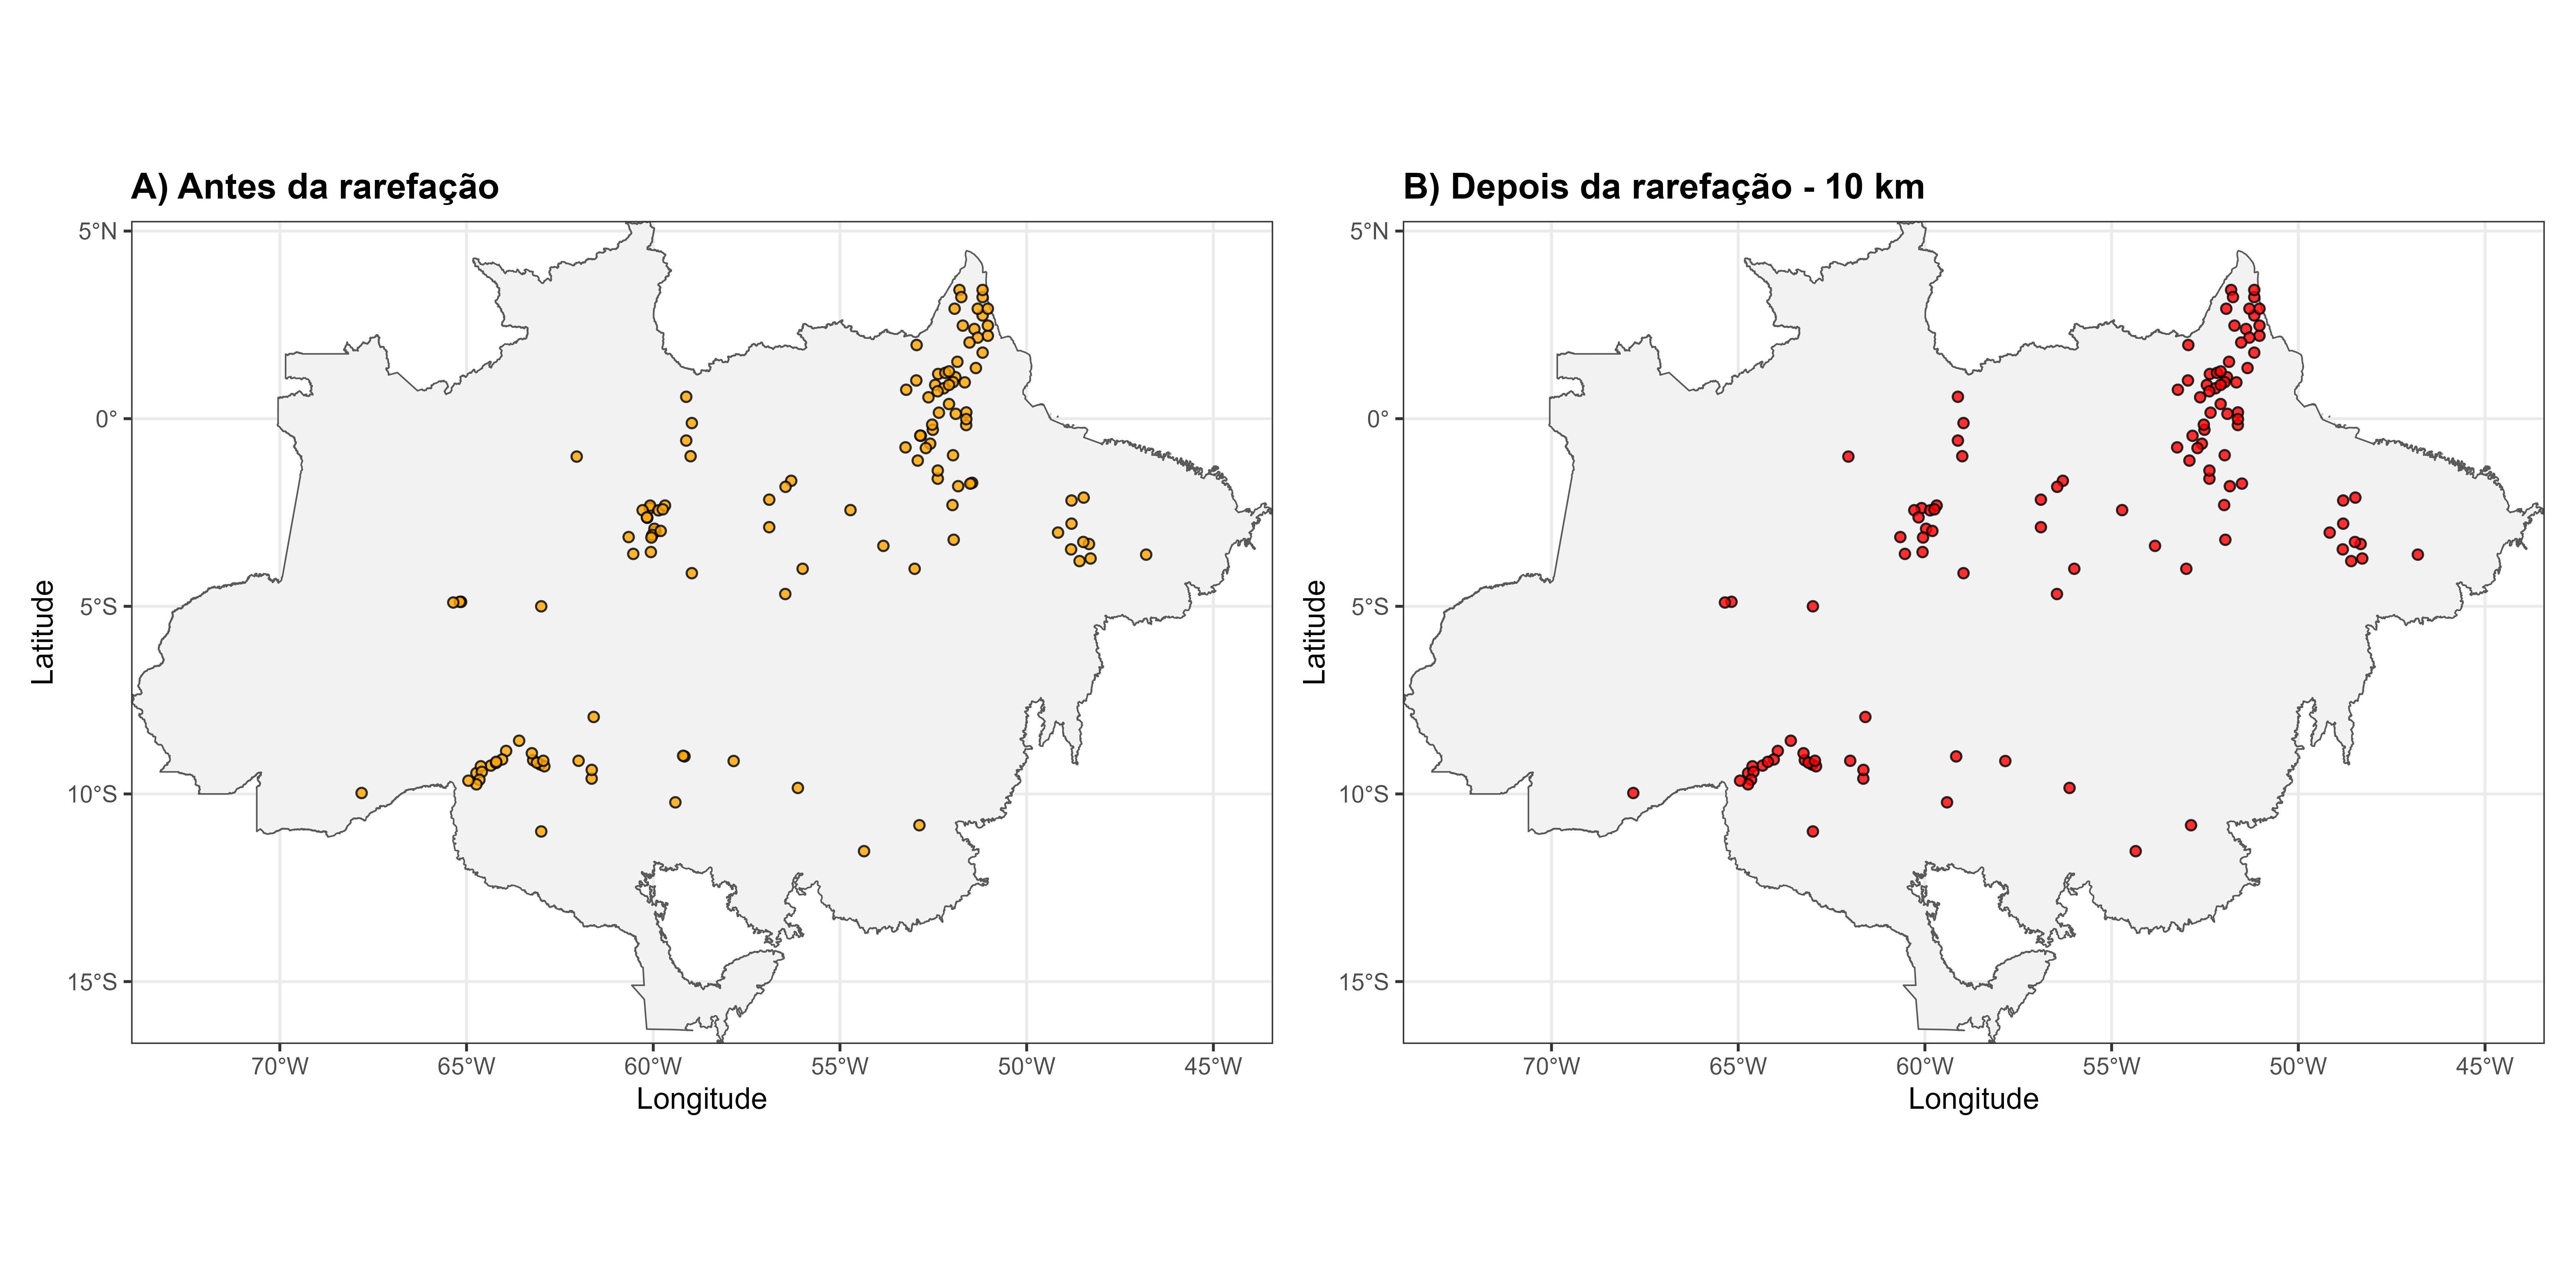
\includegraphics[width=0.92\textwidth]{figuras/unidade02/unidade02_rarefacao_dinizia.png}
  \caption{Effect of spatial thinning on records of \textit{Dinizia excelsa}. The procedure reduces spatial redundancy and concentrations of nearby points.}
  \label{fig:unidade02_rarefacao_dinizia}
\end{figure}

\section{Environmental Diagnostics of the Records}

After cleaning and thinning, the final occurrences are associated with the
selected environmental variables. This step characterizes the climatic range
occupied by the species, identifies extreme values, and prepares the final
matrix for model fitting.

\rscriptfile{scripts/unidade02/05_diagnostico_ambiental_dinizia.R}

\begin{figure}[H]
  \centering
  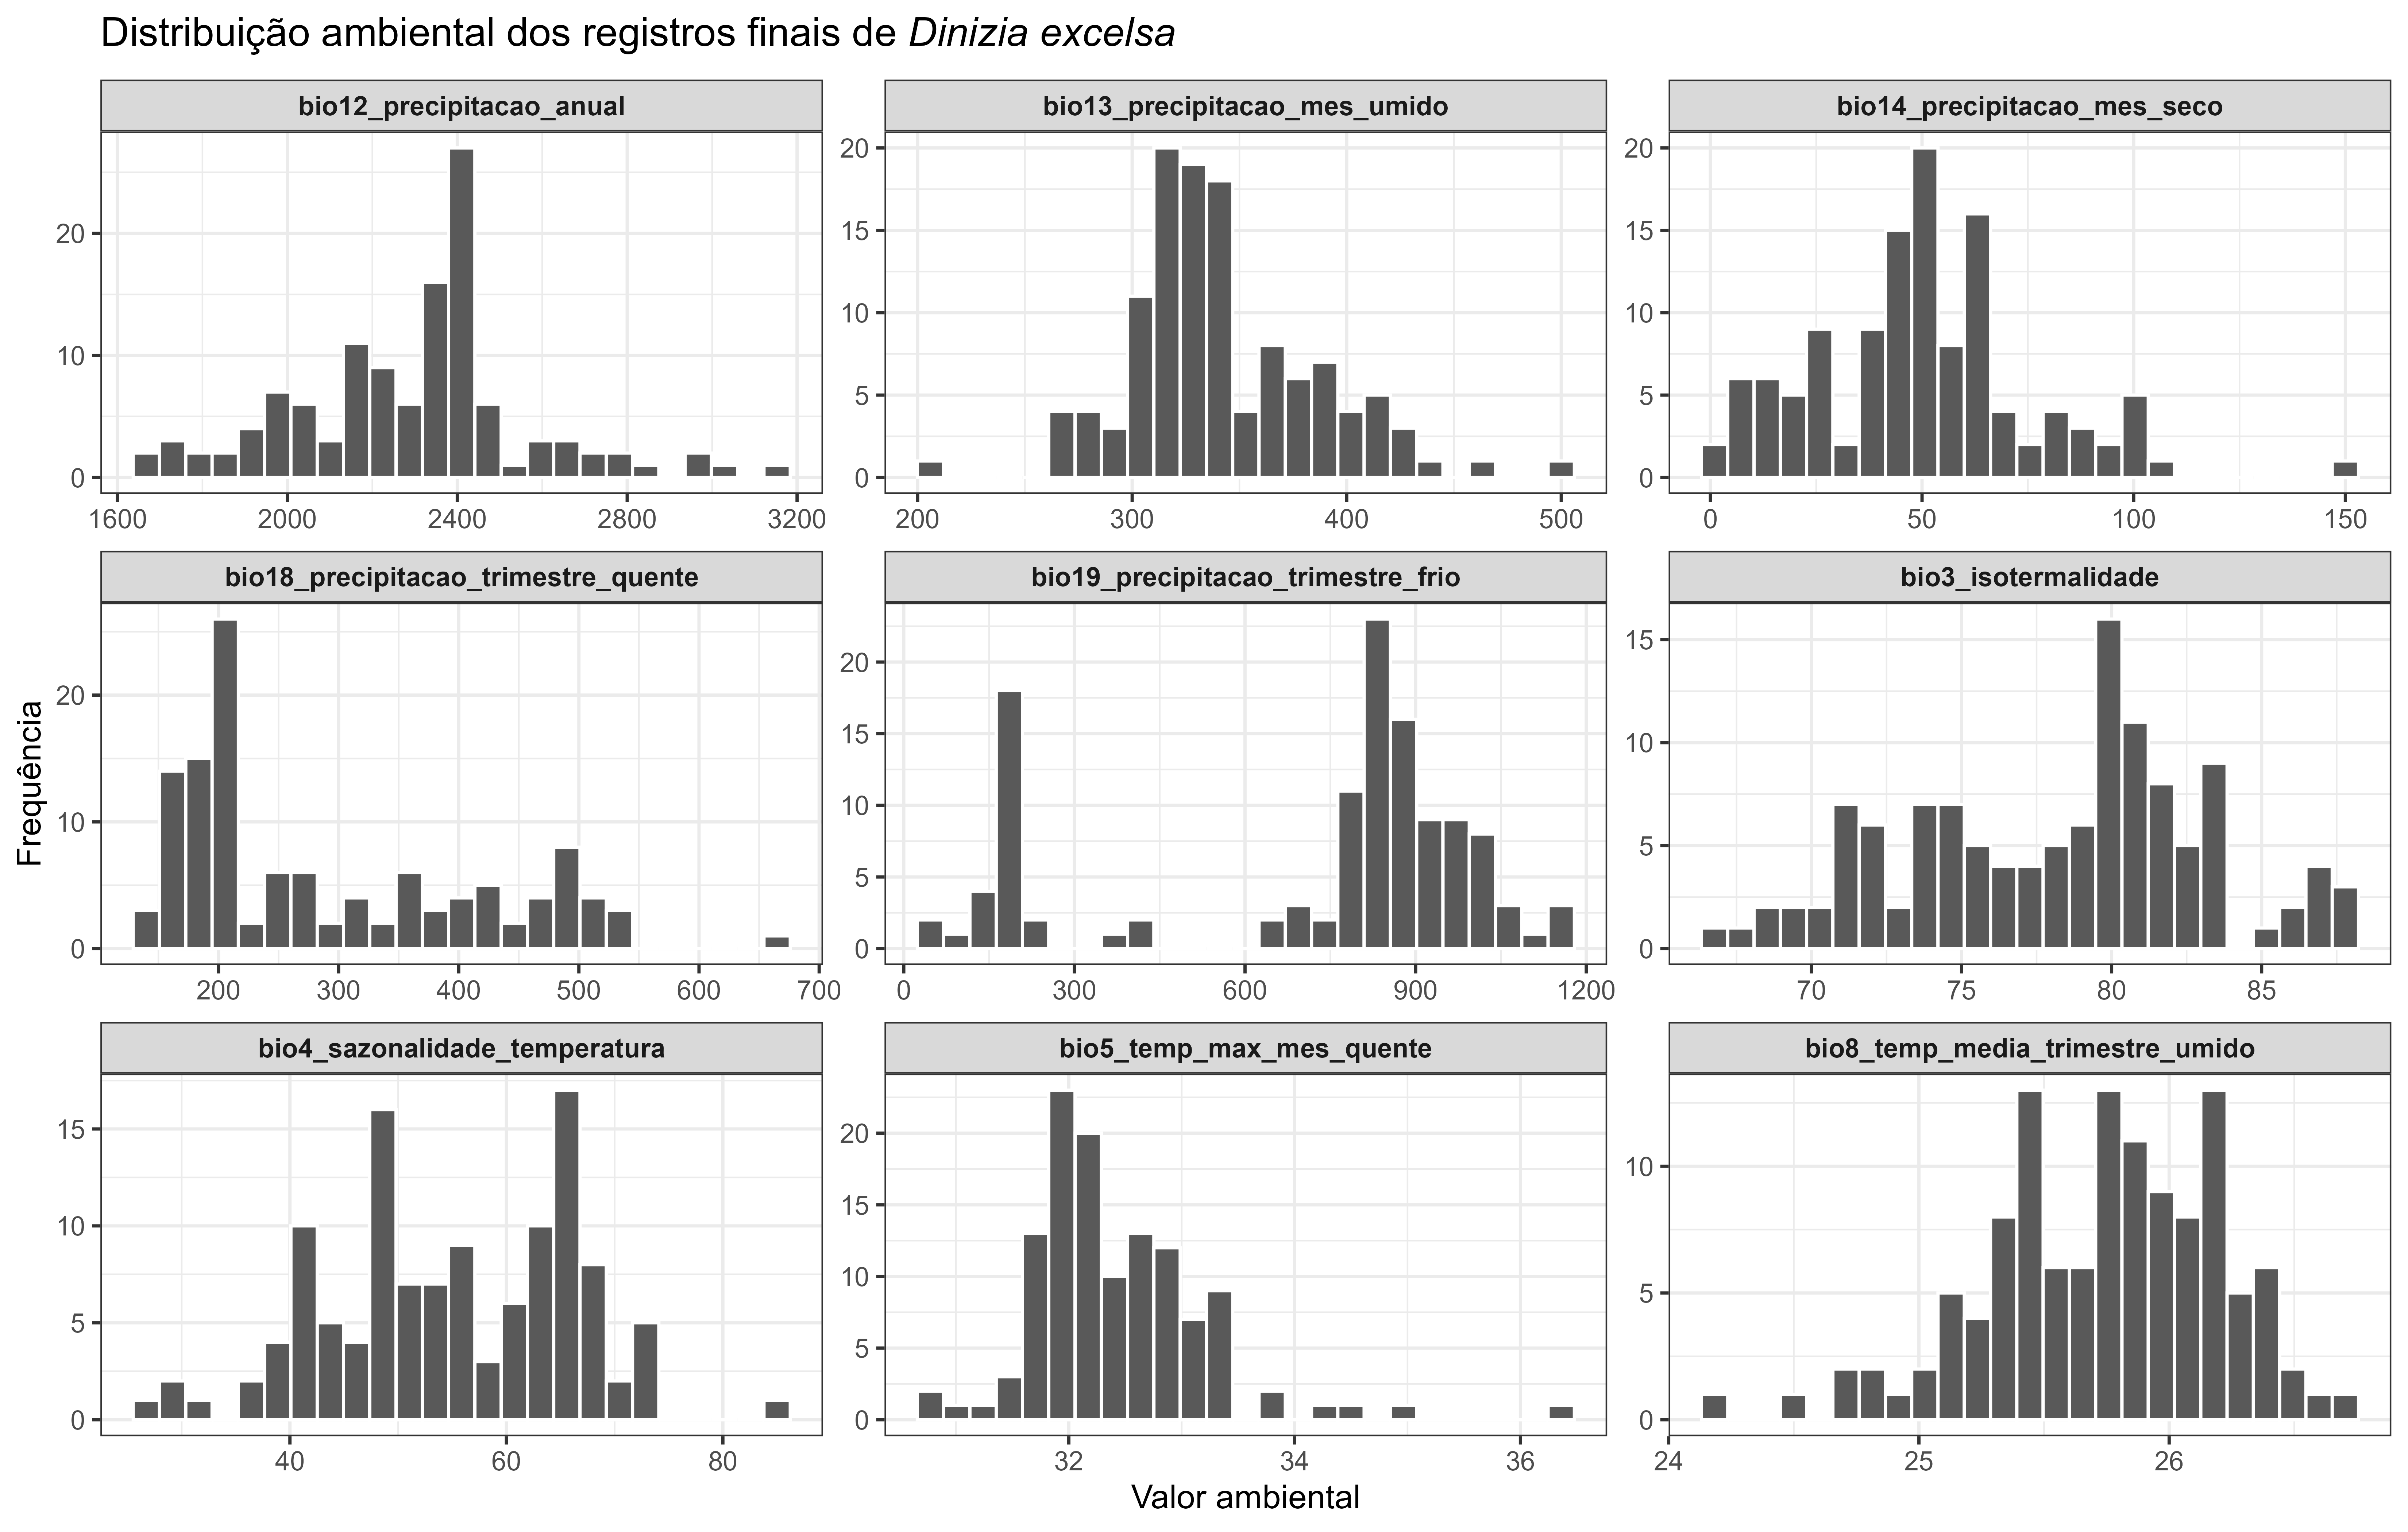
\includegraphics[width=0.92\textwidth]{figuras/unidade02/unidade02_histogramas_variaveis_dinizia.png}
  \caption{Distributions of bioclimatic variables extracted at the final \textit{Dinizia excelsa} occurrence locations.}
  \label{fig:unidade02_hist_variaveis_dinizia}
\end{figure}

\begin{figure}[H]
  \centering
  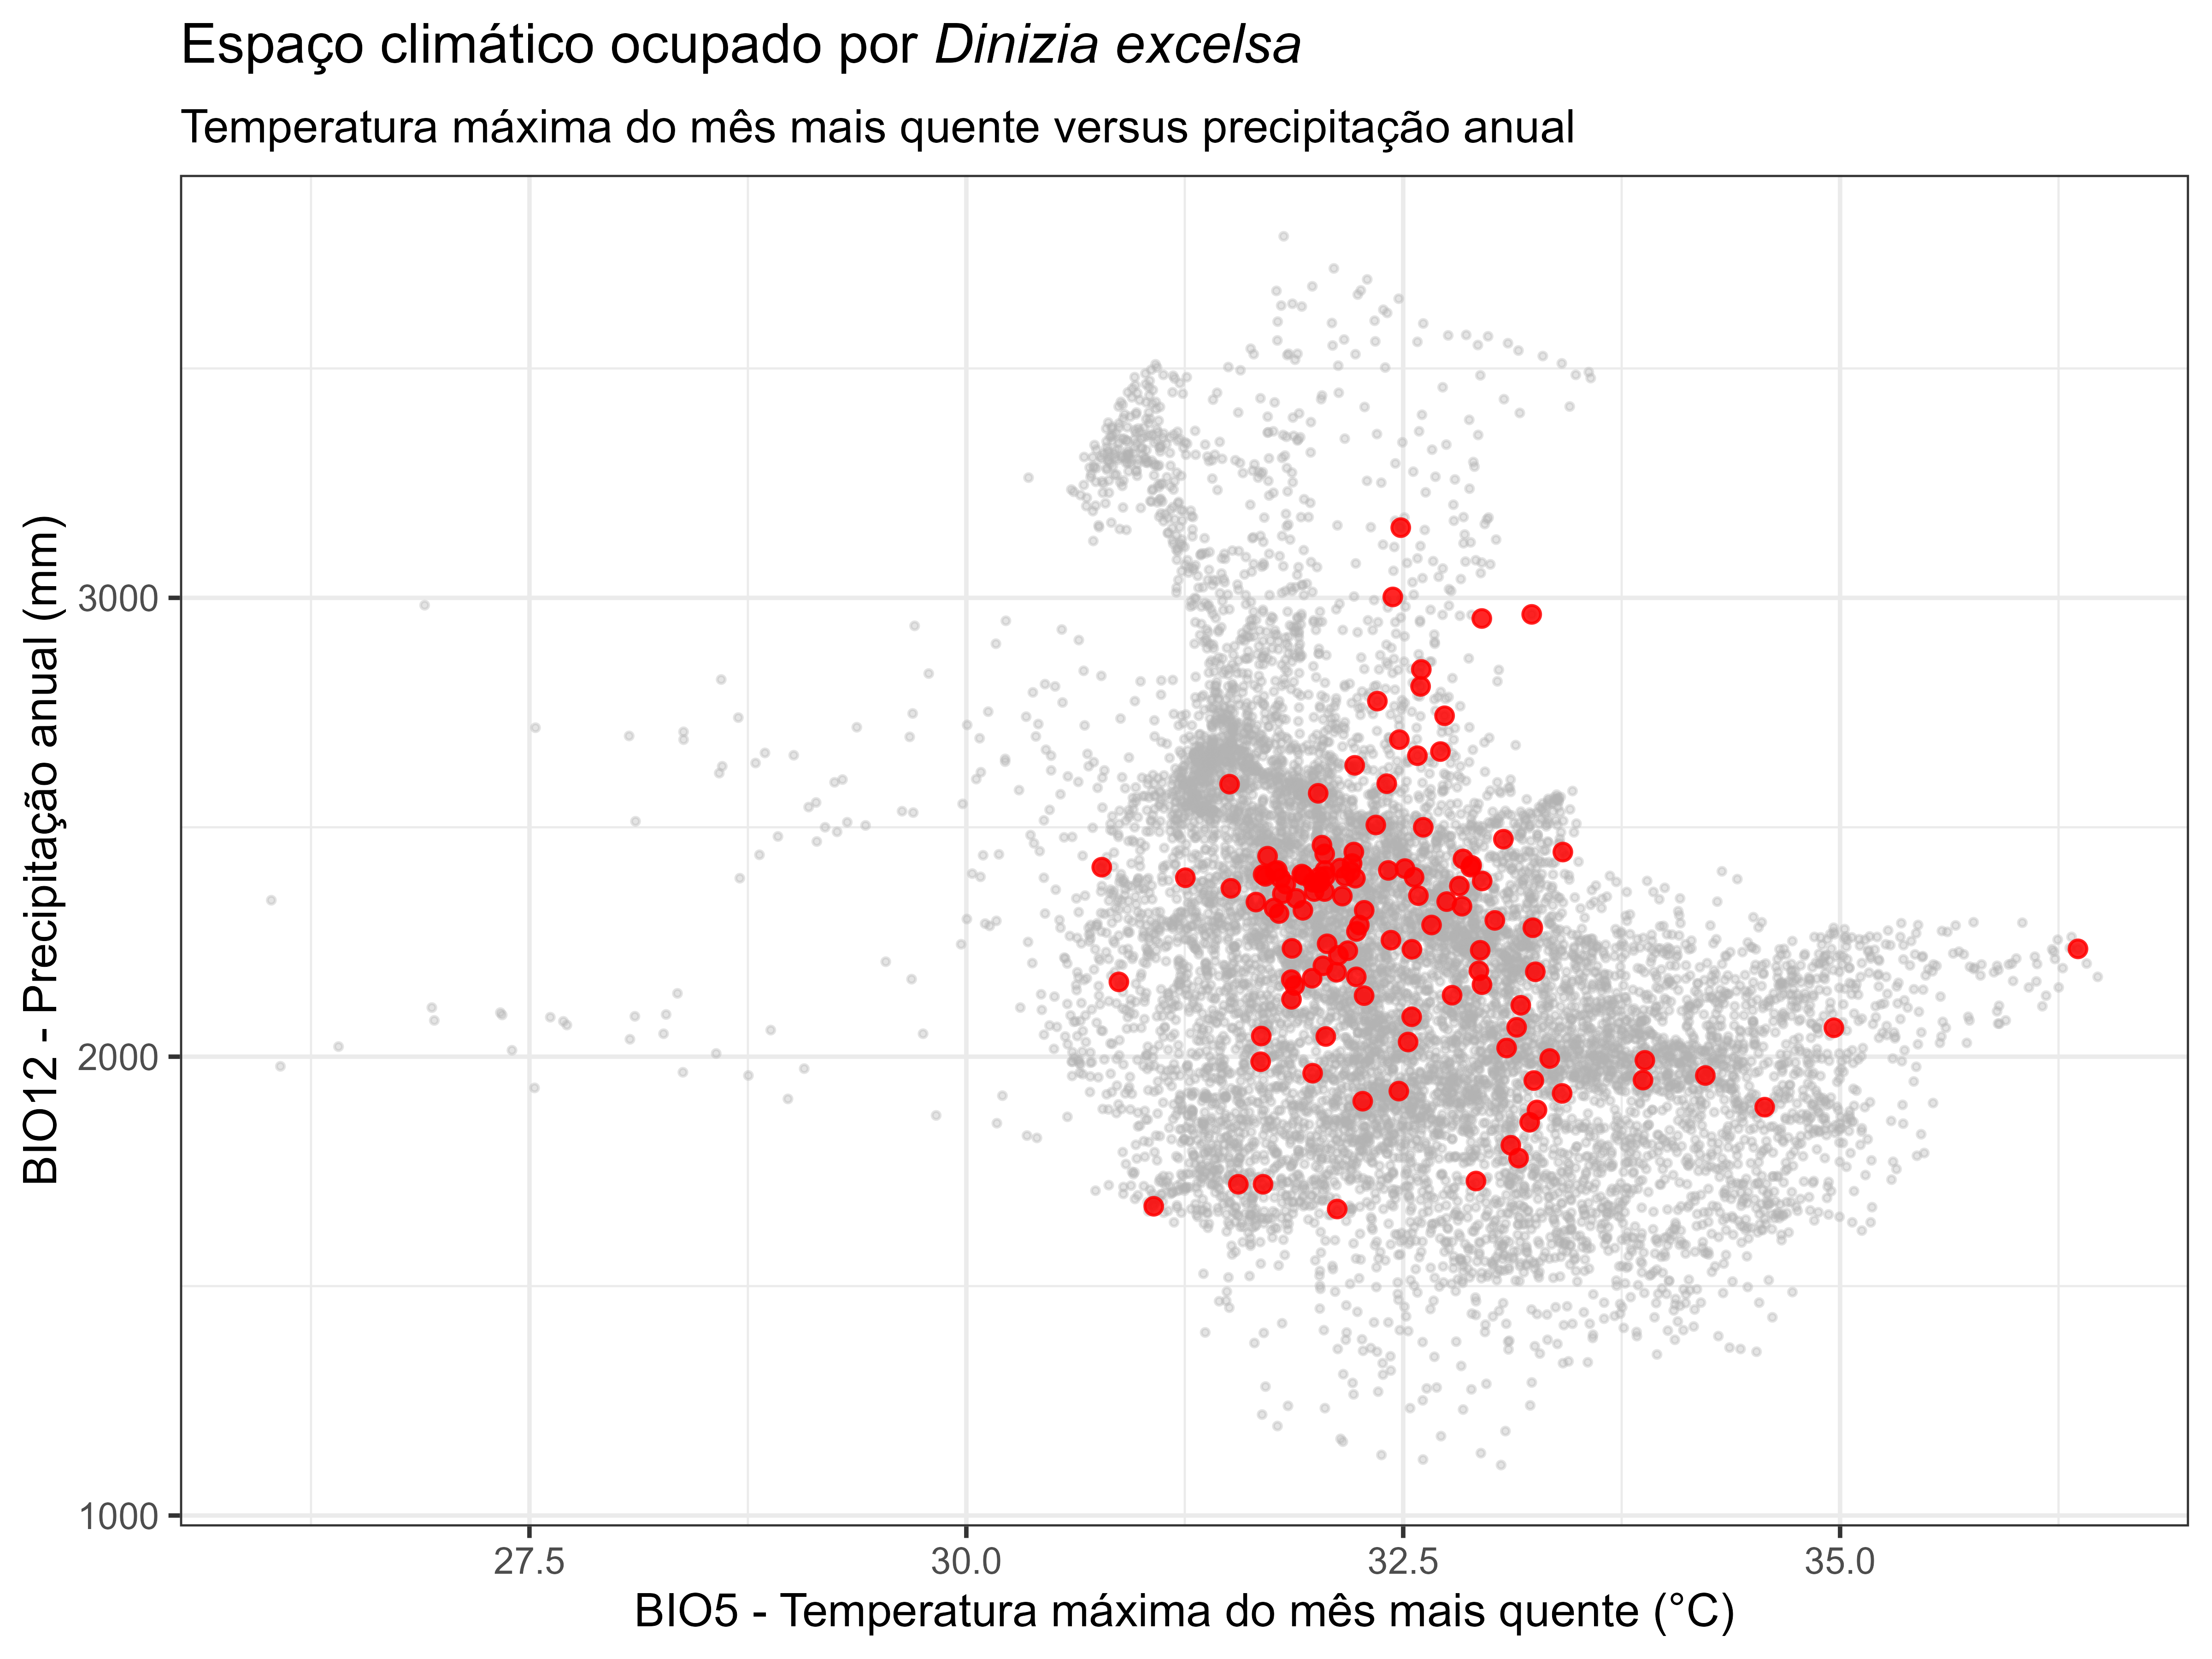
\includegraphics[width=0.86\textwidth]{figuras/unidade02/unidade02_espaco_climatico_dinizia.png}
  \caption{Climatic space occupied by \textit{Dinizia excelsa} relative to the environmental background of the Amazon biome.}
  \label{fig:unidade02_espaco_climatico_dinizia}
\end{figure}

\section{Processing Flowchart}

The flowchart summarizes the decisions used to transform raw occurrence
records into a modeling-ready dataset.

\rscriptfile{scripts/unidade02/06_fluxograma_preparacao_dinizia.R}

\begin{figure}[H]
  \centering
  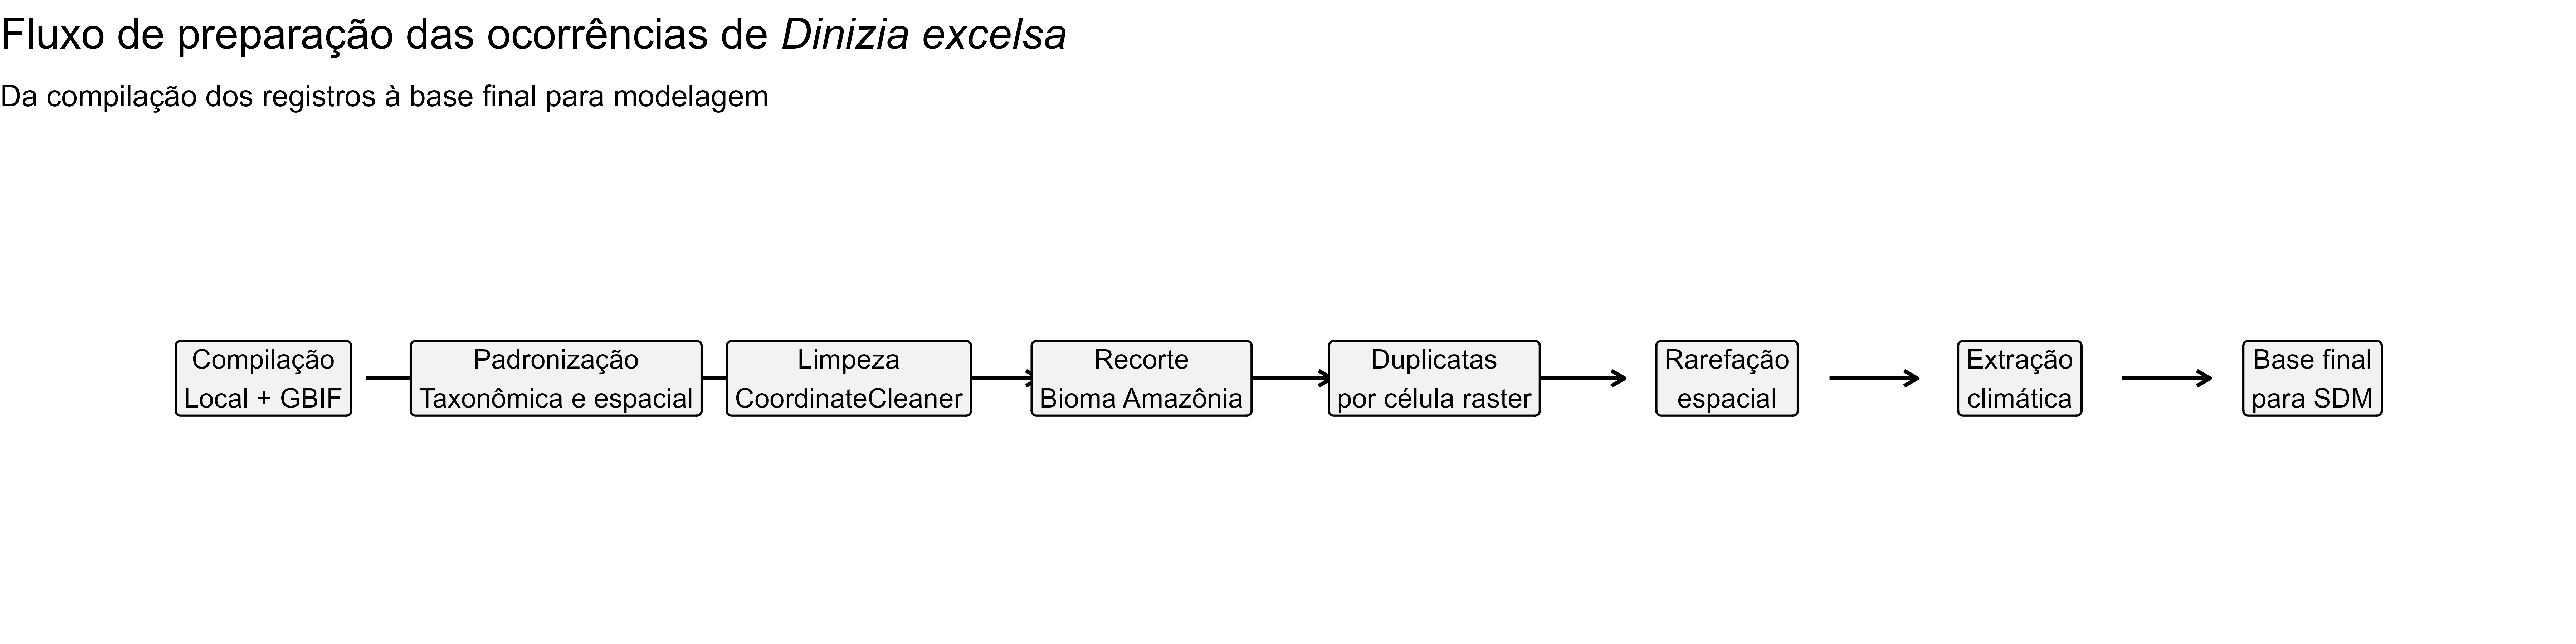
\includegraphics[width=0.92\textwidth]{figuras/unidade02/unidade02_fluxograma_preparacao_dinizia.png}
  \caption{Occurrence-data preparation workflow for SDM, using \textit{Dinizia excelsa} as a case study.}
  \label{fig:unidade02_fluxograma_dinizia}
\end{figure}

\section{Complete Chapter 2 Pipeline}

\rscriptfile{scripts/unidade02/07_pipeline_unidade02_dinizia.R}

\section{Chapter Summary}

Preparing occurrence data is one of the most important stages of SDM.
Sophisticated models cannot compensate for poor data. Final model quality
depends on taxonomic consistency, spatial validity, duplicate control,
reduction of sampling bias, and compatibility between the occurrence records
and environmental variables.

\begin{conceito}[title={\faBook\quad Key message}]
Before fitting any algorithm, raw records must be transformed into a clean,
spatially coherent, environmentally consistent occurrence dataset that matches
the scale of the study.
\end{conceito}

\section{Review Exercises}

\begin{enumerate}
  \item Explain why GBIF and herbarium records must be cleaned before modeling.
  \item Distinguish a geographic duplicate from a raster-cell duplicate.
  \item Why should records outside the study biome be removed?
  \item Explain the purpose of spatial thinning.
  \item What is sampling bias in SDM?
  \item Why should a lack of records not automatically be interpreted as species absence?
  \item Propose a cleaning workflow for a rare Amazonian tree species.
\end{enumerate}
